\documentclass{article}
\usepackage{amsmath}
\usepackage{amsfonts}
\usepackage{amsthm}
\usepackage{tikz}
\usepackage{algorithm2e}
\usepackage{fancyhdr}
\usepackage{extramarks}

%
% Homework Details
%   - Title
%   - Due date
%   - Class
%   - Section/Time
%   - Instructor
%   - Author
%

\newcommand{\hmwkTitle}{Homework\ \#1}
\newcommand{\hmwkDueDate}{February 14, 2020}
\newcommand{\hmwkClass}{MECH7710: Optimal Estimation and Control}
\newcommand{\hmwkClassInstructor}{Dr. Martin}
\newcommand{\hmwkAuthorName}{\textbf{Matthew Boler}}

%
% Homework Problem Environment
%
% This environment takes an optional argument. When given, it will adjust the
% problem counter. This is useful for when the problems given for your
% assignment aren't sequential. See the last 3 problems of this template for an
% example.
%

\setcounter{secnumdepth}{0}
\newcounter{partCounter}
\newcounter{homeworkProblemCounter}
\setcounter{homeworkProblemCounter}{1}
\nobreak\extramarks{Problem \arabic{homeworkProblemCounter}}{}\nobreak{}

\newcommand{\enterProblemHeader}[1]{
    \nobreak\extramarks{}{Problem \arabic{#1} continued on next page\ldots}\nobreak{}
    \nobreak\extramarks{Problem \arabic{#1} (continued)}{Problem \arabic{#1} continued on next page\ldots}\nobreak{}
}

\newcommand{\exitProblemHeader}[1]{
    \nobreak\extramarks{Problem \arabic{#1} (continued)}{Problem \arabic{#1} continued on next page\ldots}\nobreak{}
    \stepcounter{#1}
    \nobreak\extramarks{Problem \arabic{#1}}{}\nobreak{}
}

\newenvironment{homeworkProblem}[1][-1]{
    \ifnum#1>0
        \setcounter{homeworkProblemCounter}{#1}
    \fi
    \section{Problem \arabic{homeworkProblemCounter}}
    \setcounter{partCounter}{1}
    \enterProblemHeader{homeworkProblemCounter}
}{
    \exitProblemHeader{homeworkProblemCounter}
}

\setcounter{MaxMatrixCols}{20} % allow larger matrices

%
% Matlab code envs 
%

\usepackage{fancyvrb}
\fvset{formatcom=\color{blue},fontseries=c,fontfamily=courier,xleftmargin=4mm,commentchar=!}
\DefineVerbatimEnvironment{Code}{Verbatim}{formatcom=\color{blue},fontseries=c,fontfamily=courier,fontsize=\footnotesize,xleftmargin=4mm,commentchar=!}
\DefineVerbatimEnvironment{CodeSmall}{Verbatim}{formatcom=\color{blue},fontseries=c,fontfamily=courier,fontsize=\scriptsize,xleftmargin=1mm,commentchar=!}
\DefineVerbatimEnvironment{CodeNum}{Verbatim}{numbers=left,numbersep=4pt,formatcom=\color{blue},fontseries=c,fontfamily=courier,fontsize=\footnotesize,xleftmargin=4mm}

\newcommand{\var}[1]{{\color{blue}\Verb+#1+}}
\newcommand{\model}[1]{\index{code}{#1@\textit{#1}}\ifthenelse{\boolean{draft}}{{\color{green}\Verb+#1+}}{\Verb+#1+}}
\newcommand{\block}[1]{\ifthenelse{\boolean{draft}}{{\color{green}\Verb+#1+}}{\textsf{#1}}}
\newcommand{\func}[2][ZZZZ]{\ifthenelse{\equal{#1}{ZZZZ}}{\index{code}{#2}}{\index{code}{#1}}\ifthenelse{\boolean{draft}}{{\color{green}\Verb+#2+}}{\Verb+#2+}}
\newcommand{\methodb}[2]{\index{code}{#1@\textbf{#1}!.#2}\ifthenelse{\boolean{draft}}{{\color{magenta}\Verb+#1.#2+}}{\Verb+#1.#2+}}
\newcommand{\method}[2]{\index{code}{#1@\textbf{#1}!.#2}\ifthenelse{\boolean{draft}}{{\color{magenta}\Verb+#2+}}{\Verb+#2+}}
\newcommand{\class}[1]{\index{code}{#1@\textbf{#1}}\ifthenelse{\boolean{draft}}{{\color{cyan}\Verb+#1+}}{\Verb+#1+}}
\newcommand{\property}[1]{\index{property}{#1}\ifthenelse{\boolean{draft}}{{\color{cyan}\Verb+#1+}}{\Verb+#1+}}

\newcommand{\MATLAB}{MATLAB\textsuperscript{\textregistered}}

%
% Basic Document Settings
%

\topmargin=-0.45in
\evensidemargin=0in
\oddsidemargin=0in
\textwidth=6.5in
\textheight=9.0in
\headsep=0.25in

\linespread{1.1}
\pagestyle{fancy}
\lhead{\hmwkAuthorName}
\chead{\hmwkClass: \hmwkTitle}
\rhead{\firstxmark}
\lfoot{\lastxmark}
\cfoot{\thepage}

\title{
    \vspace{2in}
    \textmd{\textbf{\hmwkClass:\ \hmwkTitle}}\\
    \normalsize\vspace{0.1in}\small{Due\ on\ \hmwkDueDate}\\
    \vspace{3in}
}

\author{\hmwkAuthorName}
\date{}


\begin{document}

\maketitle
\pagebreak


\begin{homeworkProblem}
    Use the \MATLAB convolve function to produce discrete PDFs for throws of six dice as follows:

    \begin{enumerate}
        \item[a] 6 numbered 1, 2, 3, 4, 5, 6
        \item[b] 6 numbered 4, 5, 6, 7, 8, 9
        \item[c] 6 numbered 1, 1, 3, 3, 3, 5
        \item[d] 3 numbered 1, 2, 3, 4, 5, 6 and 3 numbered 1, 1, 3, 3, 3, 5
    \end{enumerate}

    \textbf{Solution}

    The PDFs of each are shown below:
    
    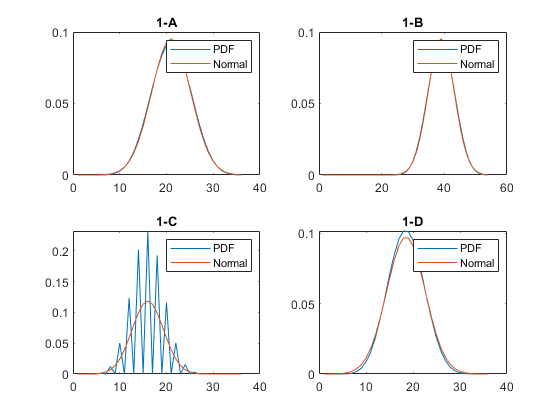
\includegraphics[]{p1}

\end{homeworkProblem}

\begin{homeworkProblem}
    \begin{enumerate}
        \item[a] What is the PDF for 2 fair dice?
        \item[b] What are $E(X_1)$, $E(X_1 - E(X_1))$, $E(X_1^2)$, $E((X_1 - E(X_1))^2)$, and $E(((X_1 - E(X_1))*(X_2 - E(X_2))))$?
        \item[c] Form the covariance matrix for $x_1$ and $x_2$
        \item[d] Find the PDF matrix for $V_1 = x_1$ and $v_2 = x_1 + x_2$
        \item[e] What is the mean, $E(v_1 - E(v_1))$, rms, and variance of $v_1$?
        \item[f] What is the mean, $E(v_2 - E(v_2))$, rms, and variance of $v_2$?
        \item[g] What is the new covariance matrix?
    \end{enumerate}

    \textbf{Solution}
    The PDF for two dice can be represented as the following matrix:
    \begin{align*}
        \frac{1}{6^2}*ones(6,6)
    \end{align*}

    \begin{align*}
        E(X_1) &= \sum xf(x) = 3.5 \\
        E(X_1 - E(X_1)) &= E(X_1) - E(X_1) = 0 \\
        E(X_1^2) &= \sum x_1^2f(x_1) = 15.167 \\
        E[(X_1 - E(X_1))^2] &= \sum(x_1 - E(X_1))^2 f(x) = 2.916 \\
        E[(X_1 - E(X_1)) * (X_2 - E(X_2))] &= \sum \sum (x_1 - E(X_1)(x_2 - E(X_2)))f(x_1, x_2) = 2.916 
    \end{align*}
    
    \begin{align*}
        Cov(X_1, X_2) = \begin{bmatrix}
            \sigma_{x_1}^2 = 2.916 & E[X_1X_2]] - E[X_1]E[X_2] = 0 \\
            E[X_1X_2]] - E[X_1]E[X_2] = 0 & \sigma_{x_2}^2 = 2.916
        \end{bmatrix}
    \end{align*}

    The PDF for $V_1 = X_1$ and $V_2 = X_1 + X_2$ is ($V_1 \in [1,6]$ on rows, $V_2 \in [2,12]$ on columns)
    \begin{align*}
        \frac{1}{6^2} \begin{bmatrix}
            1&1&1&1&1&1&0&0&0&0&0\\
            0&1&1&1&1&1&1&0&0&0&0\\
            0&0&1&1&1&1&1&1&0&0&0\\
            0&0&0&1&1&1&1&1&1&0&0\\
            0&0&0&0&1&1&1&1&1&1&0\\
            0&0&0&0&0&1&1&1&1&1&1
        \end{bmatrix}
    \end{align*}

    \begin{align*}
        E[v_1] &= E[x_1] = 3.5 \\
        E[v_1 - E(v_1)] &= E[x_1] - E[x_1] = 0 \\
        rms_{v_1} &= \sqrt{\sum v_1^2 f(v_1)} = 3.89 \\
        \sigma_{v_1}^2 &= E[(v_1)^2] - E[v_1]^2 = 2.916
    \end{align*}

    \begin{align*}
        E[v_2] &= E[x_1 + x_2] = E[x_1] + E[x_2] = 7 \\
        E[v_2 - E(v_2)] &= 0 \\
        rms_{v_2} &= \sqrt{\sum v_2^2 f(v_2)} =  \sqrt{(E[v_2]^2 + \sigma_{v_2}^2)} = 9.11 \\
        \sigma_{v_2}^2 &= \sigma_{x_1} + \sigma_{x_2} = 5.832
    \end{align*}

\end{homeworkProblem}

\begin{homeworkProblem}
    Two random vectors $X_1$ and $X_2$ are uncorrelated if 
    
    \begin{align*}
        E[(X_1 - \overline{X_1})(X_2 - \overline{X_2})] = 0
    \end{align*}

    Show that:
    \begin{enumerate}
        \item Independent random vectors are uncorrelated
        \item Uncorrelated Gaussian random vectors are independent
    \end{enumerate}

    \textbf{Solution}
    If two random vectors are independent, then $f(x_1, x_2) = f(x_1)f(x_2)$.
    From this we get 
    \begin{align*}
        E[X_1X_2] &= \sum \sum x_1 x_2 f(x_1) f(x_2) \\
        &= \sum x_1 f(x_1) \sum x_2 f(x_2) \\
        &= E[X_1]E[X_2]
    \end{align*}
    Since $Cov(X_1, X_2) = E[X_1X_2] - E[X_1]E{X_2} = 0$, the vectors are uncorrelated.

    If two gaussian random vectors are uncorrelated, then $\rho_{1,2} = 0$.
    From this, the exponential term in the PDF takes the form $\exp(\alpha_1 X_1^2 + \alpha_2 X_2^2)$, which can clearly be written as a separable product of exponentials, and the vectors are thus independent.
\end{homeworkProblem}

\begin{homeworkProblem}
    Consider a sequence created by throwing a pair of dice and summing the numbers, which are $[-2.5, -1.5, -0.5, 0.5, 1.5, 2.5]$.
    Call this $V_0(k)$.
    \begin{enumerate}
        \item[a] What is the PDF?
        \item[b] What are the mean and variance?
    \end{enumerate}
    If we generate a new random sequence
    \begin{align*}
        V_N(k+1) = (1-r)V_N(k) + rV_0(k),
    \end{align*}
    $V_N(k)$ is serially correlated.
    \begin{enumerate}
        \item[c] What are the steady-state mean and variance of this new sequence?
        \item[d] What is the covariance function $R(k) = E[V_N(k)V_N(k-L)]$?
        \item[e] Are there any practical constrains on $r$?
    \end{enumerate}

    \textbf{Solution}
    
    \begin{align*}
        f(v_0) &= 
        \frac{1}{6^2}
        \begin{bmatrix}
            1&2&3&4&5&6&5&4&3&2&1
        \end{bmatrix} \in [-5,5] \\
        E[v_0] &= 0 \\
        \sigma_{v_0}^2 &= 5.832
    \end{align*}

    If we expand the sequence definition backwards in time a few steps, we find that it is described by the summation
    \begin{align*}
        V_n(k) = (1-r)^k V_0(0) + \sum_{i = 0}^{k - 1} r(1-r)^iV_0(i)
    \end{align*}

    Our $V_0(0)$ term goes to 0 as $k\rightarrow\inf$, and
    \begin{align*}
        E[ \sum_{i=0}^{k-1}r(1-r)^i V_0(i)] &= rE[V_0]\sum_{i=0}^{k-1}(1-r)^i \\
        &= 0
    \end{align*}

    Performing the same expansion for $V_n(k)^2$, we get
    
    \begin{align*}
        V_n(k)^2 = (1-r)^{2k}V_n(0)^k + \sum_{i=0}^{k-1}r^2(1-r)V_0(i)^2
    \end{align*}

    Again, our $V_0(0)$ term goes to 0, and
    \begin{align*}
        E[ \sum_{i=0}^{k-1} r^2(1-r)^{2i}V_0(i)^2] &= r^2 \sum_{i=0}^{k-1} (1-r)^{2i} E[V_0(i)^2] \\
        &= [r^2 \sum_{i=0}^{k-1} (1-r)^{2i}] (\sigma_{v0}^2 - 0)
    \end{align*}

    From these,
    \begin{align*}
        \sigma_{vn}^2 &= E[V_n^2] - E[V_n]^2 \\
        &= \sigma_{v0}^2 [r^2 \sum_{i=0}^{k-1} (1-r)^{2i}]
    \end{align*}


    To find $R(L)$ we'll start with a small example where $L=1$.
    \begin{align*}
        E[V_N(k)V_N(k-1)] &= E[ ((1-r)V_N(k-1) + rV_0(k-1)) * V_N(k-1) ] \\
        &= E[ (1-r)V_N(k-1)^2 ] + E[ rV_0(k-1)V_N(k-1) ] \\
        &= (1-r)E[V_N(k-1)^2]
    \end{align*}
    From this, we expand the general solution to $R(L) = (1-r)^L E[V_N(k-L)^2]$.
    There's still some work to be done in exactly solving back to $V_N(1)$, but this gets the general idea that the sequence is less correlated with itself over larger time steps.
    A practical constraint on $r$ is that $|r| \in [0,1]$, otherwise the sequence goes to infinity.

\end{homeworkProblem}

\begin{homeworkProblem}
    A random variable $x$ has a PDF given by
    \begin{align*}
        f_X = \begin{cases}
            0 & x < 0 \\
            \frac{x}{2} & 0 \leq x < 2 \\
            0 & x \geq 2
        \end{cases}
    \end{align*}
    \begin{enumerate}
        \item[a] What is the mean of $x$?
        \item[b] What is the variance of $x$? 
    \end{enumerate}

    \textbf{Solution}

    \begin{align*}
        \mu_x &= \int_{0}^{2} x\frac{x}{2}dx \\
        &= \frac{x^3}{6}|_0^2 \\
        &= \frac{4}{3}
    \end{align*}

    \begin{align*}
        \sigma_x^2 &= E[X^2] - E[X]^2 \\
        &= \int_0^2x^2\frac{x}{2}dx - \frac{16}{9} \\
        &= \frac{x^4}{8}|_0^2 - \frac{16}{9} \\
        &= 2 - \frac{16}{9}
    \end{align*}
\end{homeworkProblem}

\begin{homeworkProblem}
    Consider a normally-distributed 2D vector $X$, with mean $0$ and 
    \begin{align*}
        P_X = \begin{bmatrix}
            2 & 1 \\
            1 & 4
        \end{bmatrix}
    \end{align*}
    \begin{enumerate}
        \item[a] Find the eigenvalues of $P_X$
        \item[b] What are the principal axes?
        \item[c] Plot the likelihood ellipses for $c = 0.25, 1, 1.5$
        \item[d] What is the probability of finding $X$ inside each of these ellipses?   
    \end{enumerate}

    \textbf{Solution}
    
    \begin{Code}
        [V, D] = eig(P_x); 
        % Eigenvalues:
        D = 1.5858      0
            0           4.4142
        % Principal axes:
        V = -0.9239     0.3827
            0.3827      0.9239
    \end{Code}

    We find our error ellipses via:
    \begin{Code}
        function [c] = error_ellipse(covariance, k)
            theta = linspace(0, 2*pi, 100);
            a = k*[cos(theta); sin(theta)];
            [V, D] = eig(covariance);
            A = D^(-1/2) * V;
            A_inv = pin(A);
            c = A_inv * a;
        end
    \end{Code}
    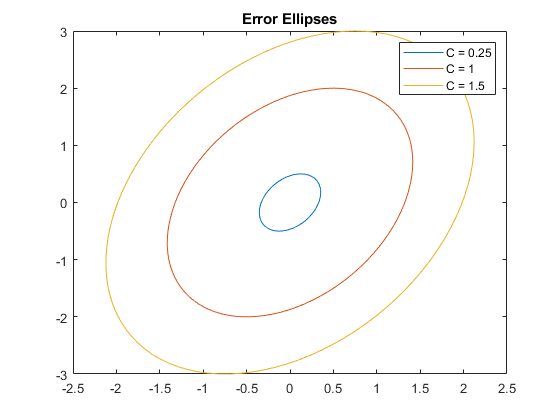
\includegraphics[]{error}

    We expect these ellipses to contain $X$ with the following probabilities:

    \begin{Code}
        c = [0.25; 1; 1.5];
        alpha = c .^ 2
        P = chi2cdf(alpha, 2);
    \end{Code}

    \begin{align*}
        C = 0.25 : P(X) = 0.0308 \\
        C = 1.00 : P(X) = 0.3935 \\
        C = 1.50 : P(X) = 0.6753
    \end{align*}

\end{homeworkProblem}

\begin{homeworkProblem}
    Given $x \sim N(0, \sigma_x^2)$ and $y = 2x^2$
    \begin{enumerate}
        \item[a] Find the PDF of $y$
        \item[b] Draw the PDFs of $x$ and $y$ on the same plot for $\sigma_x^2 = 2.0$
        \item[c] How is the density function changed by this transformation?
        \item[d] Is $y$ a normal random variable?   
    \end{enumerate}
    
    \textbf{Solution}
    For an RV $X ~ N(0, \sigma_x^2)$ transformed as $Y = g(X) = 2X^2$, we slightly abuse the density transformation technique:
    \begin{align*}
        f_y(y) = |\frac{d}{dy} g^{-1}(y)| f_x(g^{-1}(y))
    \end{align*}

    To use this, $g$ must be invertible.
    Instead we will handle it piecewise for $x < 0$ and $x > 0$.

    \begin{align*}
        g^{-1}(y) &= \pm sqrt(\frac{y}{2}) \\
        | \frac{d}{dy}g^{-1}(y)| &= \frac{1}{2sqrt(2y)} \\
        f_x(x) &= \frac{1}{sqrt(2 \pi \sigma_x^2)}exp( \frac{-1}{2} (\frac{x-\mu}{\sigma})^2 ) \\
    \end{align*}

    To handle our uninvertible transformation, we only performt the calculation for $x>0$ and double it to account for $x<0$ mapping to the same value as their positive equivalent.
    \begin{align*}
        f_y(y) &= 2 * |\frac{1}{2sqrt(2y)}| f_x(sqrt(\frac{y}{2})) \\
        &= \frac{1}{2 \sigma_x sqrt(\pi y)}exp(\frac{-y}{4\sigma_x^2})
    \end{align*}

    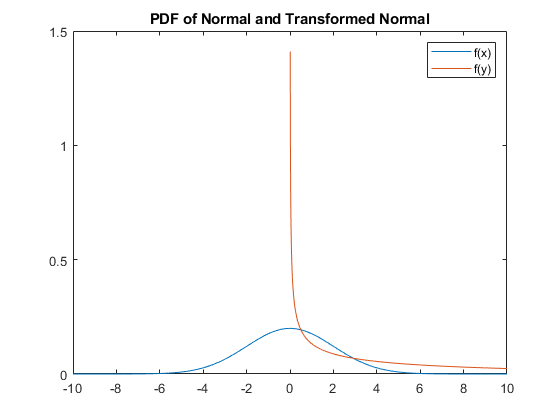
\includegraphics[]{p7.png}

\end{homeworkProblem}
    
\end{document}